\documentclass[tikz]{standalone}
\usepackage{tikz}
\usepackage{fourier}
\usepackage{physics}
\usetikzlibrary{shapes.geometric}
\usetikzlibrary{calc}

\begin{document}
\begin{tikzpicture}
    % Spherical harmonic plots
    \node[inner sep=0] at (0, 0) {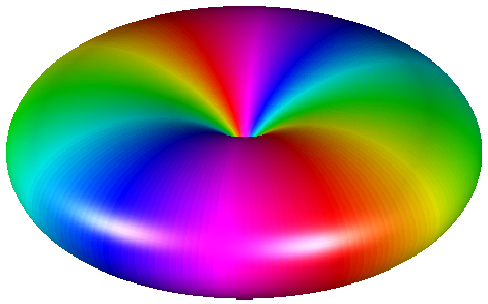
\includegraphics{../gfx/FM-2-spherical.pdf}};
    \node[inner sep=0] at (8, 0) {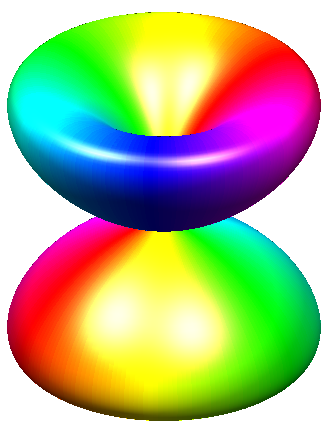
\includegraphics{../gfx/FM-1-spherical.pdf}};
    \node[inner sep=0] at (16, 0) {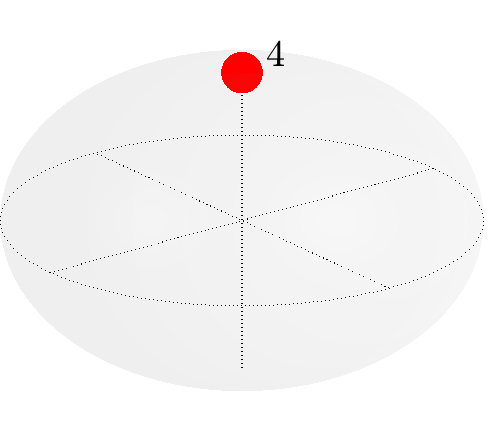
\includegraphics{../gfx/FM-2-Majorana.pdf}};
    \node[inner sep=0] at (25, 0) {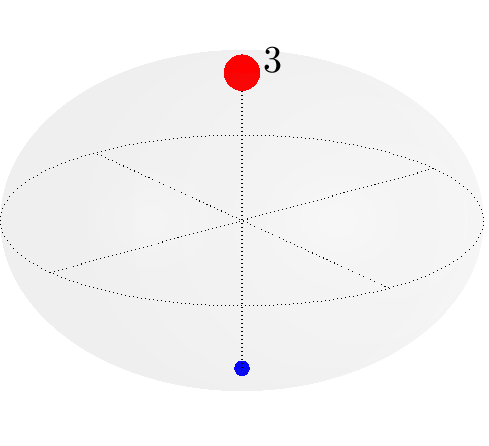
\includegraphics{../gfx/FM-1-Majorana.pdf}};

    % Colour bar
    \node[rotate=90] at (-5, 0) {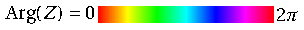
\includegraphics[scale=1.8]{../gfx/compiled_hsv.pdf}};
    \node at (30, 0) {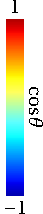
\includegraphics[scale=1.8]{../gfx/compiled_jet_majorana.pdf}};

    % Labels
    \node at (-0.1, -4.5) {\Huge (a)};
    \node at (8, -4.5) {\Huge (b)};
    \node at (16, -4.5) {\Huge (c)};
    \node at (25, -4.5) {\Huge (d)};

    % FM labels
    \draw[->, dashed, line width=2] (0, 0.25) -- (0, 3) node[above] {\Huge \(\langle\hat{\vb{F}}\rangle\)};
    \draw[->, dashed, line width=2] (8, 1.3) -- (8, 3.8) node[above] {\Huge \(\langle\hat{\vb{F}}\rangle\)};

    % Orientation
    \draw[->, line width=2] (-4, -4) -- (-4, -3) node[above] {\Huge \(z\)};
    \draw[->, line width=2] (-4, -4) -- (-3, -4) node[right] {\Huge \(x\)};
    \draw[->, line width=2] (-4, -4) -- (-3.4, -3.5) node[right] {\Huge \(y\)};

    % Spinor labels
    \node at (16, 3.7) {\Huge \(\zeta^{\text{FM}_2} = (1, 0, 0, 0, 0)^T\)};
    \node at (25, 3.7) {\Huge \(\zeta^{\text{FM}_1} = (0, 1, 0, 0, 0)^T\)};

\end{tikzpicture}
\end{document}

